%\subsection{Effect of lens radium}
%lensed_waveguide_radium
In this part we are going to fixed height of the lens on the waveguide and change the lens radium.
In Tab. \ref{ tab:coupling_lensed_waveguide_radium} the lens height is choosed for $1\mu$m, $1.5\mu$m and $2\mu$m respectively. Change the lens radium from $2\mu$m to $3.6\mu$m and observe $|S21|$ as coupling efficiency.

\begin{table}
\caption{Cupling efficiency between TLF and lensed waveguide due to changing the lens radium}
\begin{tabular}{|c|c|c|c|}
\hline
Radium($\mu$m)|Height($\mu$m)&	1&	1.5&2\\
\hline
$2.0$& $59.5\%$	&$61.3\%$	&$69\%$\\
$2.2$& $59\%$		&$60.8\%$	&$68.3\%$\\
$2.4$&$59\%$		&$60.3\%$	&$66.8\%$\\
$2.6$&$58.6\%$	&$59.9\%$	&$65.3\%$\\
$2.8$&$58.2\%$	&$59.3\%$	&$64\%$\\
$3.0$&$57.8\%$	&$58.7\%$	&$63\%$\\
\hline
\end{tabular}
\label{tab:coupling_lensed_waveguide_radium}
\end{table}
Map the the data into a Fig. \ref{fig:coupling_lenses_curve_hxx}
\begin{figure}[!ht]
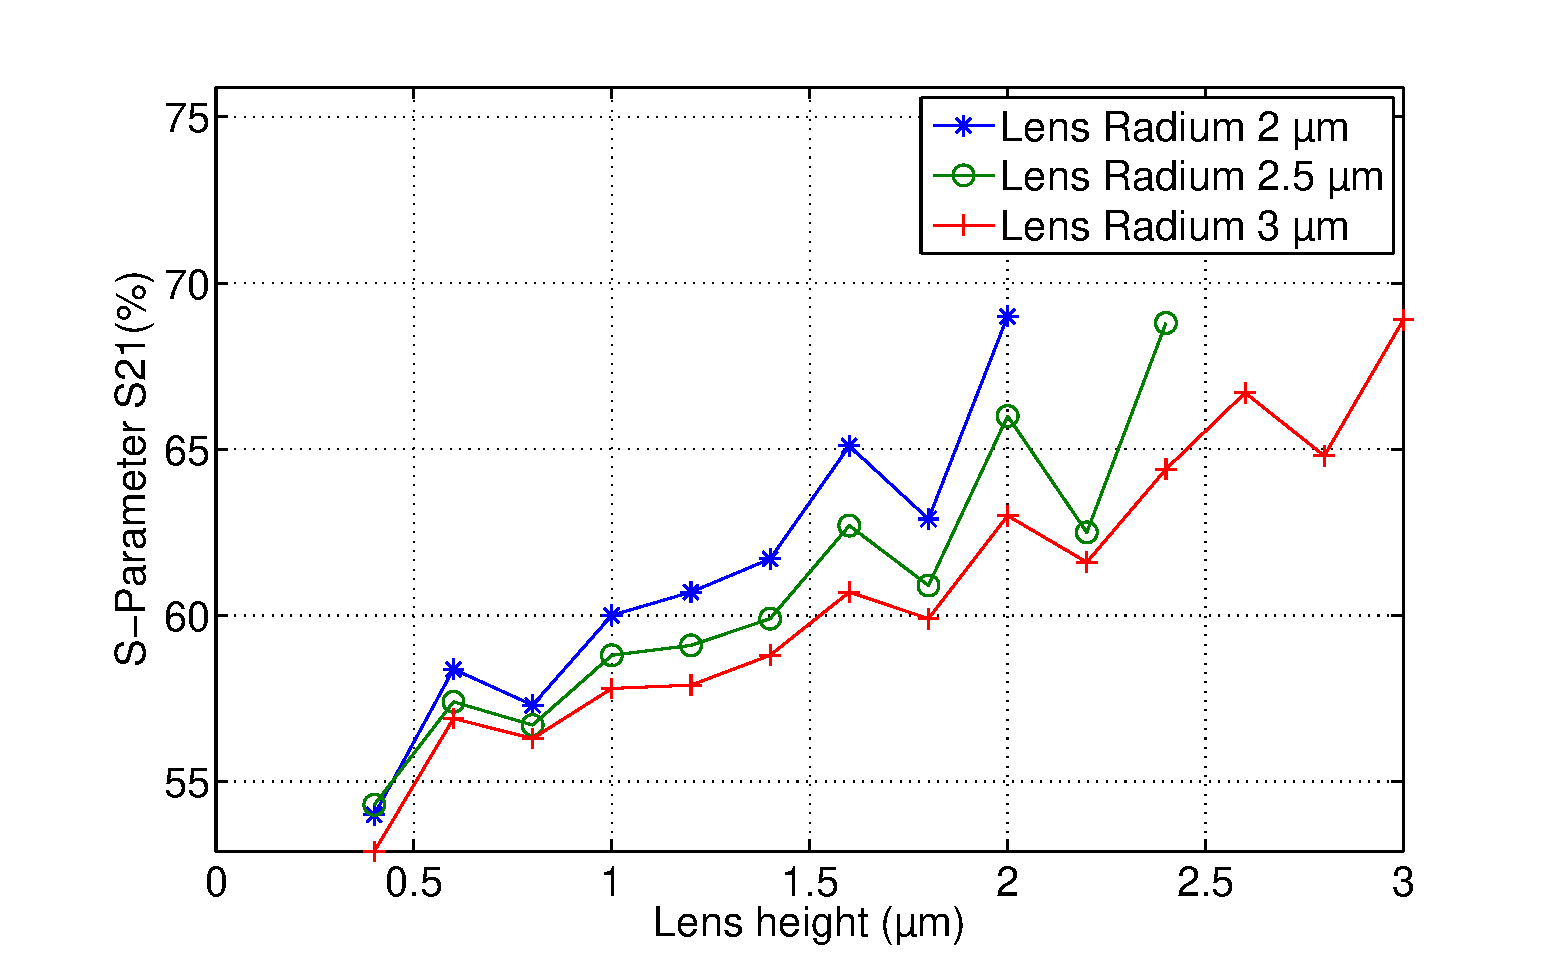
\includegraphics[width=0.8\textwidth]{bilder/s21_fix_lens_radium_hxx}
\caption{Coupling efficiency due to changing the lens radium}
\label{fig: coupling_lenses_curve_hxx}
\end{figure}


\begin{figure}[!ht]
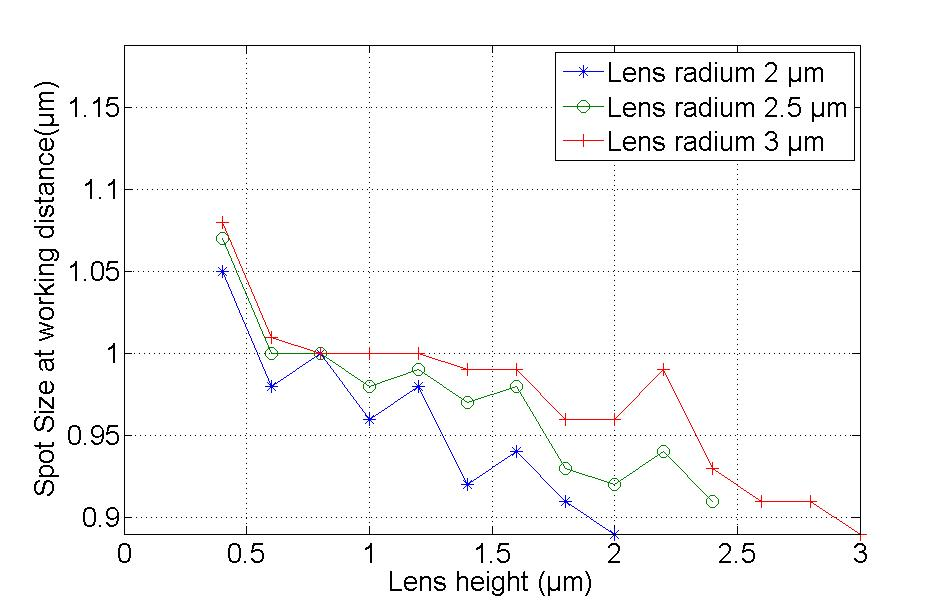
\includegraphics[width=0.8\textwidth]{bilder/spot_fix_lens_radium_hxx}
\caption{The spot size curve at lensed waveguide interface due to changing lens height}
\label{fig: fig: lensed_guide_spot_size_ curve}
\end{figure}
